\subsection{Why Care about Software Architecture?}

% Clone and own from SE1 09a
\begin{frame}{Architecture Bridges the Gap}
	\begin{fancycolumns}[columns=3,animation=none]
		\uncover<4->{
			\begin{example}{}
				Large software systems \ldots
				\begin{itemize}
					\item have numerous requirements
					\item require many developers
					\item need separation of concerns\\\deutsch{Trennung von Belangen}
				\end{itemize}
			\end{example}
		}
		\nextcolumn
		\nextcolumn
		\uncover<3->{
			\begin{note}{}
				\mycite{Weeks of coding can save you hours of planning.}\mysource{anon}
			\end{note}
		}
	\end{fancycolumns}
	\begin{tikzpicture}[xscale=4.95]
		\node[label=below:Requirements] (req) at (0,0) {\pic[height=2.5cm]{architecture/requirements}};
		\only<2->{\node[label=below:Implementation] (code) at (2,0) {\pic[height=2.5cm]{architecture/source-code}};}
		%\only<2>{\node[label=below:Softwarearchitektur] (swa) at (.95,0) {\includegraphics[height=1.9cm]{component-diagram}};}
		\only<5->{
			\draw[->,line width=5pt,gray] (req) -- (code);
			\node[label=below:Software Architecture] (swa) at (.95,0) {\pic[height=2.5cm]{architecture/component-diagram-large}};
		}
	\end{tikzpicture}
\end{frame}

% Clone and own from SE1 09a
\begin{frame}{\insertsubsection\ \normalsize[\sommerville]}
	\begin{fancycolumns}[columns=1] % hack to make mindmap visible in dark mode
		\centering{\tikz[grow cyclic,
				mindmap, every node/.style=concept,concept color=red!20!background,
				%text width=20mm,align=flush center,
				level 1/.append style={level distance=27mm,sibling angle=360/3}]
			\node {Goals of Software Architectures}
			[clockwise from=210]
			child[visible on=<2->] { node {meet critical requirements} }
			child[visible on=<3->] { node {communication of stakeholders} }
			child[visible on=<4->] { node {support software reuse} }
			;}
	\end{fancycolumns}
\end{frame}

% Clone and own from SE1 09a
\begin{frame}[10]{Architecture Design in the Software Development Process}
	\begin{fancycolumns}[widths={45}]
		\diagramWaterfallModel
		\nextcolumn
		\diagramVModel
	\end{fancycolumns}
\end{frame}

\subsection{What is Software Architecture?}

% TODO: replace this
\begin{frame}{\insertsubsection\ \mytitlesource{\sommerville}}
	\begin{fancycolumns}[keep]
		\begin{definition}{Architectural Design \deutsch{Architekturentwurf}}
			\mycite{\emph{Architectural design} is a creative process in which you design a system organization that will satisfy the functional and non-functional requirements of a system.}
		\end{definition}
		\pause
		\begin{definition}{Software Architecture}
			\mycite{A \emph{software architecture} is a description of how a software system is organized. Properties of a system such as performance, security, and availability are influenced by the architecture used.}
		\end{definition}
		\nextcolumn
		\pause
		\begin{example}{In Practice:}
			\mycite{You might propose an abstract system architecture where you associate groups of system functions or features with large-scale components or subsystems. You then use this decomposition to discuss the requirements and more detailed features of the system with stakeholders.}
		\end{example}
	\end{fancycolumns}
\end{frame}

\subsection{What to Consider When Designing Software Architecture?}

\begin{frame}
	\frametitle{Properties of Software Systems to Consider \mytitlesource{\sommerville}}
	\begin{fancycolumns}[widths={50,50}]
		\begin{definition}{Performance}
			Tackling performance via architecture design:
			\begin{itemize}
				\item Larger components $\rightarrow$ fewer cross-component interactions
				\item Option to scale via replication/distribution of components
			\end{itemize}
		\end{definition}
		\begin{definition}{Maintainability}
			Tackling maintainability via architecture design:
			\begin{itemize}
				\item Smaller dedicated components $\rightarrow$ separation of concerns, easier to understand and modify
				\item Option to replace components without affecting the rest of the system
			\end{itemize}
		\end{definition}
		\nextcolumn
		\begin{definition}{Safety}
			Tackling safety via architecture design:
			\begin{itemize}
				\item Couple safety critical operations in very few components $\rightarrow$ simplify verification
			\end{itemize}
		\end{definition}
		\begin{definition}{Security}
			Tackling security via architecture design:
			\begin{itemize}
				\item Critical assets in low layers $\rightarrow$ not accessible to outer layers
			\end{itemize}
		\end{definition}
		\begin{definition}{Availability}
			Tackling availability via architecture design:
			\begin{itemize}
				\item Redundancy via replication of components
				\item Backup strategy
			\end{itemize}
		\end{definition}

	\end{fancycolumns}


\end{frame}

\begin{frame}{Architectural Views \mytitlesource{\sommerville}}
	\begin{fancycolumns}[keep]
		{\tikz[grow cyclic,
				mindmap, every node/.style=concept,concept color=blue!20!background,
				%text width=20mm,align=flush center,
				level 1/.append style={level distance=27mm,sibling angle=360/4}]
			\node {Architectural Views}
			[clockwise from=225]
			child[visible on=<2->] { node {logical view} }
			child[visible on=<3->] { node {process view} }
			child[visible on=<4->] { node {development view} }
			child[visible on=<5->] { node {physical view} }
			;}
		\nextcolumn
		\begin{motivation}{Why Views? \mysource{\sommerville}}
			\small
			\mycite{It is impossible to represent all relevant information about a system's architecture in a single architectural model.}
		\end{motivation}
		\begin{definition}{Different Views \mysource{Kruchten (4+1)}}
			\small
			\begin{itemize}
				\item \emph{Logical}: Key abstractions fulfilling functional requirements
				\item \emph{Process}: Composition of system in interacting processes $\rightarrow$ examine non-functional requirements such as performance and availability
				\item \emph{Development}: Software modularization: partitioning, grouping, visibility $\rightarrow$ Maintainability, reusability
				\item \emph{Physical}: Underlying hardware and network layout $\rightarrow$ performance, availability, reliability
			\end{itemize}
		\end{definition}
	\end{fancycolumns}
\end{frame}